\documentclass[12pt, a4paper]{article}

\usepackage[brazil]{babel}
\usepackage[
    letterpaper,
    top=2cm, bottom=2cm,
    left=2cm, right=2cm
]{geometry}

\usepackage{amsmath}
\usepackage{amsthm}
\usepackage{graphicx}
\usepackage{mathpazo}
\usepackage[colorlinks=true, allcolors=blue]{hyperref}
\usepackage[square,numbers]{natbib}
\usepackage{blindtext}
\usepackage{xcolor}
\usepackage{soul}
\usepackage{braket}
\usepackage{indentfirst}

\usepackage{tikz}
\usetikzlibrary{positioning}

\newtheorem{theorem}{Teorema}[section]
\newtheorem{definition}{Definição}[section]
\newtheorem{lemma}{Lema}[section]

\hypersetup{
    colorlinks=true,       % false: boxed links; true: colored links
    linkcolor=blue,          % color of internal links (change box color with linkbordercolor)
    citecolor=black,        % color of links to bibliography
    filecolor=black,      % color of file links
    urlcolor=purple           % color of external lin
}

\title{Trabalho de Matemática Discreta\\
\Large{Matchings e ciclos hamiltonianos em grafos de hipercubos}}

\author{
    Amanda Perez \\
    Juan Belieni
}

\date{
    FGV/EMAp \\
    \today
}

\begin{document}

\maketitle

\section{Introdução}

Desde o início dos tempos, os seres humanos empreendem grandes esforços para responder algumas perguntas fundamentais: quem somos nós? por que estamos aqui? há vida após a morte? Por não termos os meios de responder nenhuma dessas perguntas, vamos apresentar neste trabalho a demonstração da conjectura de que todo \textit{matching} perfeito em grafos de hipercubo pode ser estendido em um ciclo hamiltoniano.

Este problema, resolvido apenas em 2007~\cite{fink_perfect_2007}, é uma versão mais fraca de uma conjectura que permanece sem solução, que afirma que qualquer \textit{matching} em um hipercubo consegue ser estendido em um ciclo hamiltoniano.

Ao longo das próximas seções, buscamos apresentar as principais definições envolvidas nesse problema, bem como provar propriedades relevantes. O objetivo é que este material possa ser tanto uma introdução ao tópico quanto um sumário de definições e teoremas.

\section{Grafos de hipercubos}

Nesta seção, definimos grafos de hipercubos e suas principais propriedades. Um grafo de hipercubo pode ser entendido intuitivamente como um grafo construído sobre um hipercubo $d$-dimensional (ou $d$-cubo), onde os vértices e arestas do grafo representam, respectivamente, os vértices e arestas do hipercubo.

\begin{definition}[Definição de grafo de hipercubo I] \label{def:hyper-i}
    O {\bf grafo de hipercubo} $d$-dimensional $Q_d = (V, E)$ é o grafo onde $V$ são todas as sequências $( p_i )_{i = 1}^d$, onde $p_i \in \{ 0, 1 \}$, e $\{ u, v \} \in E$ se, e somente se, $u$ e $v$ diferem em exatamente uma posição dessa sequência~\cite[p.~97]{socorro_rangel_elementos_2018}.
\end{definition}

\begin{figure}[h]
    \centering
    \begin{tikzpicture}[scale=1.4, every node/.append style={font=\footnotesize}]
        \node[draw] (v1) at (0,0) {0, 0, 0};
        \node[draw] (v2) at (2,0) {1, 0, 0};
        \node[draw] (v3) at (2,2) {1, 0, 1};
        \node[draw] (v4) at (0,2) {0, 0, 1};
        \node[draw] (v5) at (1,1) {0, 1, 0};
        \node[draw] (v6) at (3,1) {1, 1, 0};
        \node[draw] (v7) at (3,3) {1, 1, 1};
        \node[draw] (v8) at (1,3) {0, 1, 1};
    
        \draw (v1) -- (v2) -- (v3) -- (v4) -- (v1);
        \draw (v5) -- (v6) -- (v7) -- (v8) -- (v5);
        \draw (v1) -- (v5);
        \draw (v2) -- (v6);
        \draw (v3) -- (v7);
        \draw (v4) -- (v8);
    \end{tikzpicture}
    \caption{Representação gráfica de um cubo ($Q_3$), exemplificando a definição \ref{def:hyper-i}.}
    \label{fig:cube-graph}
\end{figure}

Apesar de ser bem intuitiva, a definição \ref{def:hyper-i} pode não ser tão prática quando utilizada em algumas demonstrações ou mesmo em implementações computacionais. Dessa forma, apresentamos a seguir uma definição alternativa que se utiliza do conceito de produto cartesiano em grafos para definir hipercubos recursivamente. Antes disso, contudo, definamos a operação de produto cartesiano em grafos.

\begin{definition} \label{def:cartesian-prod}
Sejam $G = (V_G, E_G)$ e $H = (V_H, E_H)$ dois grafos quaisquer. O produto cartesiano $G \times H$~\cite[p.~22]{harary_graph_2001} é o grafo $G\times H = (V', E')$, onde $V' = V_G \times V_H$ (produto cartesiano entre os conjuntos de vértices) e $E'$ é definido de modo que dois vértices $(v_G, v_H), (u_G, u_H) \in V'$ são adjacentes se, e somente se, vale exatamente uma das seguintes afirmações:
\begin{itemize}
    \item $u_G = v_G$, e $v_H$ e $u_H$ são adjacentes em $H$; ou
    \item $u_H = v_H$, e $v_G$ e $u_G$ são adjacentes em $G$.
\end{itemize}
\end{definition}

Utilizando a operação definida em \ref{def:cartesian-prod}, temos a seguinte definição alternativa para o grafo de hipercubo:

\begin{definition}[Definição de grafo de hipercubo II] \label{def:hyper-ii}
    O {\bf grafo de hipercubo} $d$-dimensional $Q_d$ pode ser definido recursivamente como $Q_d = Q_{d - 1} \times K_2$, onde $Q_1 = K_2$~\cite{harary_survey_1988}.
\end{definition}

A partir de agora, chamaremos todos os grafos de hipercubo apenas de hipercubos e vamos considerar apenas os hipercubos com dimensão $d \geq 2$. Além disso, vamos demonstrar que as duas definições dadas são equivalentes.

\begin{lemma}\label{lemma:equiv_def}
As definições \ref{def:hyper-i} e \ref{def:hyper-ii} são equivalentes.
\end{lemma}

\begin{proof}
        A prova é por indução em $d$. O lema vale para $d = 2$.\footnote{Para verificar isso, basta notar que construindo $Q_2 = K_2 \times K_2$, com os vértices de $K_2$ nomeados como $0$ e $1$, obtemos o mesmo grafo que seria construído pela definição \ref{def:hyper-i}.}

        Considerando o hipercubo $Q_{d + 1}$, temos que o lema é verdadeiro para $Q_d$ por hipótese indutiva. Ou seja, os vértices de $Q_d$ são as sequências $(p_i)_{i=1}^{d}$, onde $p_i \in \{ 0, 1 \}$, e suas arestas incidem em vértices que diferem em exatamente uma posição.

        A partir da definição \ref{def:hyper-ii}, é possível observar que os vértices de $Q_d$ podem ser divididos em dois conjuntos $V_k(Q_{d + 1}) = \{ (v, k) \}_{v \in V(Q_d)}$, $k \in \{ 0, 1 \}$.\footnote{Observação sobre a notação: aqui e em outros momentos ao longo deste trabalho, utilizaremos $V(G)$ e $E(G)$ para referenciar, respectivamente, os conjuntos de vértices e arestas do grafo $G$.} Pela definição \ref{def:cartesian-prod}, $\{ (u, i), (v, j) \} \in E(Q_{d+1})$, $\forall \{ u, v \} \in E(Q_d)$ e $\forall i, j \in \{ 0, 1 \}$, se, e somente se,
        
        \begin{itemize}
            \item $u = v$ e $i \neq j$, onde todos os elementos da sequência são iguais a não ser pelo último; ou
            \item $u \neq v$ e $i = j$, onde $u$ e $v$ já diferem em exatamente uma única posição.
        \end{itemize}

        Portanto, ambas as definições são equivalentes.
\end{proof}

\begin{figure}[h]
    \centering
    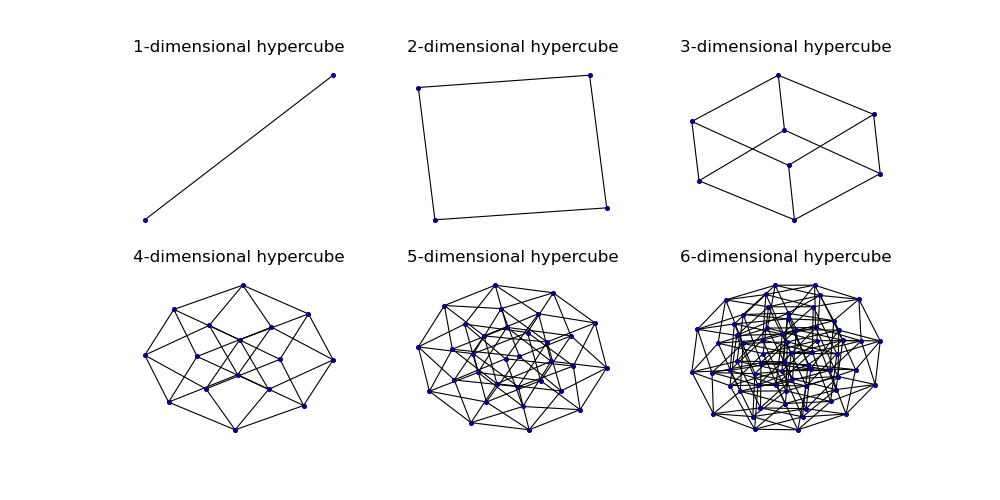
\includegraphics[width=0.95\linewidth]{figs/hypercube_examples.png}
    \caption{Grafos de hipercubo de 1 a 6 dimensões, construídos a partir da definição \ref{def:hyper-ii}. Eles foram gerados em Python com a ajuda da biblioteca \texttt{networkx}, que tem implementada a operação de produto cartesiano entre grafos. O código utilizado está disponível em: \url{https://shorturl.at/berK2}.}
    \label{fig:hypercubes}
\end{figure}

A partir dessas definições, podemos enunciar e demonstrar algumas propriedades úteis de hipercubos.

\begin{theorem}\label{teo:bipart}
    Todo hipercubo $Q_d$ é bipartido.
\end{theorem}

\begin{proof}
    Da teoria de grafos, é conhecido que um grafo $G$ é bipartido se, e somente se, todo caminho fechado em $G$ possui tamanho par. Por contradição, vamos assumir que existe um caminho fechado $p = (p_1, p_2, \dots, p_n, p_1)$ em $Q_d$, onde $n$ é um inteiro ímpar não negativo.
    
    Pela definição \ref{def:hyper-i}, conclui-se que o vértice $p_i$, com $i$ ímpar, difere de $p_1$ em um número par de posições. No entanto, $p_n$ é vizinho de $p_1$ e deveria diferir em apenas uma posição de $p_1$, acarretando uma contradição. Portanto, todo hipercubo é bipartido.
\end{proof}

Uma prova alternativa (e mais extensa) para este teorema, utilizando apenas a definição \ref{def:hyper-ii}, está apresentada no apêndice \ref{ap:prova_teo}. Ela foi omitida do texto principal por ser mais complicada em comparação com a demonstração apresentada acima, contudo sua construção será utilizada como base para demonstrar o próximo teorema.

\begin{theorem}\label{teo:hamilt}
    Todo hipercubo $Q_d$ é hamiltoniano.
\end{theorem}

\begin{proof}
    A prova será por indução em $d$. Para $d=2$, trivialmente podemos construir um ciclo hamiltoniano formado por todas as arestas de $Q_2$. 
    
    Suponha que $Q_d$ é hamiltoniano. Então, para $Q_{d+1} = Q_d \times K_2$, podemos utilizar mesma construção apresentada na prova alternativa do teorema \ref{teo:bipart} no apêndice \ref{ap:prova_teo}: considerando os subgrafos $Q'$ e $Q''$ expressos em (\ref{eq:subgrafos}), temos que ambos são isomorfos a $Q_d$. Logo, pela hipótese de indução, existe ciclo hamiltoniano em cada um deles, digamos $c_1$ e $c_2$, respectivamente; podemos escolher esses ciclos a partir de um mesmo ciclo hamiltoniano de $Q_d$, mapeando-o nos subgrafos. Nomeando os vértices de $Q_d$ de modo que $c = (v_1, v_2, \cdots, v_n, v_1)$ seja um ciclo hamiltoniano, podemos tomar $c_1 = ((v_1, 0), \cdots, (v_n, 0), (v_1, 0))$ e $c_2 = ((v_1, 1), \cdots, (v_n, 1), (v_1, 1))$.
    
    Excluindo exatamente uma aresta arbitrária de $c_1$ (digamos $\{(v_1, 0), (v_n, 0)\}$) e a equivalente em $c_2$, obtemos um caminho hamiltoniano em cada subgrafo com extremos em dois vértices vizinhos ($(v_1, 0)$ e $(v_n, 0)$ para $Q'$, e $(v_1, 1)$ e $(v_n, 1)$ em $Q''$). Por construção de $Q_{d+1}$, temos que existe uma aresta entre $(v_1, 0)$ e $(v_1, 1)$, bem como entre $(v_n, 0)$ e $(v_n, 1)$. Assim, podemos conectar os dois caminhos derivados de $c_1$ e $c_2$, formando o ciclo:
    $$
    c_{\star} = ((v_1, 0), (v_2, 0), \cdots, (v_n, 0), (v_n, 1), (v_{n-1}, 1), \cdots, (v_1, 1), (v_1, 0)).
    $$

    Por $c_1$ e $c_2$ serem ciclos hamiltonianos em $Q'$ e $Q''$ e $V(Q_{d+1}) = V(Q') \cup V(Q'')$, temos que $c_{\star}$ também é ciclo hamiltoniano. Portanto, $Q_{d+1}$ é hamiltoniano e, por consequência, todo hipercubo com $d\geq 2$.
\end{proof}


\section{\textit{Matchings} perfeitos}

O \textit{matching} (ou emparelhamento) de um grafo é entendido como um conjunto formado por arestas não adjacentes entre si\footnote{Algumas definições de \textit{matching} tem como foco principal grafos bipartidos direcionados, contudo o enfoque do trabalho não será nessa definição.}. Além disso, um \textit{matching} pode ser classificado como maximal, completo, máximo ou perfeito. Neste trabalho, iremos trabalhar principalmente com o conceito de \textit{matching} perfeito (definido em \ref{def:perfect-matching}), não apresentando, por essa razão, as definições das demais classificações citadas.

\begin{figure}[h] \label{fig:cube-graph-matching}
    \centering
    \begin{tikzpicture}[scale=1.4, every node/.append style={font=\footnotesize}]
        \node[draw] (v1) at (0,0) {0, 0, 0};
        \node[draw] (v2) at (2,0) {1, 0, 0};
        \node[draw] (v3) at (2,2) {1, 0, 1};
        \node[draw] (v4) at (0,2) {0, 0, 1};
        \node[draw] (v5) at (1,1) {0, 1, 0};
        \node[draw] (v6) at (3,1) {1, 1, 0};
        \node[draw] (v7) at (3,3) {1, 1, 1};
        \node[draw] (v8) at (1,3) {0, 1, 1};
    
        \draw[ultra thick, red] (v1) -- (v2);
        \draw[ultra thick, red] (v3) -- (v4);
        \draw[ultra thick, red] (v5) -- (v6);
        \draw[ultra thick, red] (v7) -- (v8);
        \draw (v2) -- (v3);
        \draw (v4) -- (v1);
        \draw (v6) -- (v7);
        \draw (v8) -- (v5);
        \draw (v1) -- (v5);
        \draw (v2) -- (v6);
        \draw (v3) -- (v7);
        \draw (v4) -- (v8);
    \end{tikzpicture}
    \caption{\textit{Matching} perfeito em um cubo ($Q_3$). Nessa figura, as arestas destacadas em vermelho formam um dos possíveis \textit{matchings} perfeitos de $Q_3$.}
\end{figure}

\begin{definition}
    Um \textbf{\textit{matching}} de um grafo $G = (V, E)$ é um conjunto de arestas $M \subseteq E$ tal que, $\forall x, y \in M$, $x$ e $y$ não são adjacentes entre si~\cite[p.~237]{socorro_rangel_elementos_2018}.
\end{definition}

\begin{definition}
    Seja um \textit{matching} $M$ de um grafo $G = (V, E)$ e um vértice $v \in V$. Dizemos que $v$ é \textbf{coberto} por $M$ se $\exists e \in M$ tal que $e$ incide em $v$.
\end{definition}

\begin{definition} \label{def:perfect-matching}
    Um \textbf{\textit{matching} perfeito} de um grafo $G = (V, E)$ é um \textit{matching} $P$ tal que, $\forall v \in V$, $v$ é coberto por $P$.
\end{definition}

Uma consequência direta da definição \ref{def:perfect-matching} é que não é possível construir \textit{matchings} perfeitos em grafos com uma quantidade ímpar de vértices. De fato, cada aresta do \textit{matching} incide sobre exatamente dois vértices e não é possível que mais de uma aresta incida sobre um mesmo vértice; sendo assim, um \textit{matching} cobre uma quantidade par de vértices e como não podem sobrar vértices para que ele seja perfeito, é necessário que $|V|$ seja par para que um grafo $G=(V,E)$ tenha \textit{matching} perfeito. Em particular, um hipercubo $Q_d$ tem $2^d$ vértices no total, então não é necessário considerar esse tipo de restrição ao lidarmos com hipercubos.


\section{Estendendo \textit{matchings} perfeitos de hipercubos em ciclos hamiltonianos}

Nessa seção, vamos mostrar que todo \textit{matching} perfeito de um hipercubo pode ser estendido em um ciclo hamiltoniano, o que ficou conhecido como conjectura de Kreweras~\cite{kreweras_matchings_1996} e era um problema em aberto até 2007. Para isso, vamos nos basear fortemente na demonstração presente no artigo de \citet{fink_perfect_2007}.

A intuição por trás dessa conjectura é dada pelo fato de que todo ciclo hamiltoniano em um hipercubo é composto por dois \textit{matchings} perfeitos. Isso pode ser facilmente demonstrado se consideramos que todo hipercubo é bipartido e que, consequentemente, todo caminho fechado possui tamanho par. A partir disso, podemos definir a seguinte propriedade de grafos:

\begin{definition}
    Um grafo $G$ tem a propriedade \textbf{\textit{Perfect-Matching-Hamiltonian} (PMH)} se, para cada um de seus \textit{matchings} perfeitos $P$, existe outro \textit{matching} perfeito de $P'$ tal que a $P \cup P'$ produz um ciclo hamiltoniano em $G$~\cite{abreu_perfect_2022}.
\end{definition}

Para provar que todo hipercubo possui essa propriedade, vamos primeiro enunciar um lema que servirá de passo intermediário para a demonstração final.

\begin{definition}
    Uma {\bf floresta linear} é uma floresta (ou conjunto disjunto) de árvores lineares.
\end{definition}

\begin{lemma} \label{lemma:matching-linear-forest}
    Seja $M$ um \textit{matching} não perfeito de um hipercubo $Q_d$. Então existe um \textit{matching} perfeito $P$ de $Q_d$ tal que $M \cap P = \emptyset$ e $M \cup P$ é uma floresta linear. 
\end{lemma}

\begin{proof}
    A prova é por indução em $d$. O lema vale para $d = 2$.
    
    Por $M$ não ser perfeito, então devem existir dois vértices $q_1, q_2 \in V(Q_d)$ que não são cobertos por ele. Dessa forma, é possível dividir o hipercubo $Q_d$ em dois $(d-1)$-cubos $Q^{(1)}$ e $Q^{(2)}$ tal que $q_i \in V(Q^{(i)})$, $i \in \{ 1, 2 \}$. 

    Seja $M^{(i)} = M \cap E(Q^{(i)})$, $i = \{ 1, 2 \}$, é possível concluir que $M^{(i)}$ não é perfeito, já que $q_1$ não é coberto por ele. Dessa forma, pela hipótese indutiva, existe um \textit{matching} perfeito $P^{(1)}$ de $Q^{(1)}$ tal que $M^{(1)} \cup P^{(1)}$ é uma floresta linear. Para terminar a demonstração, é necessário encontrar um \textit{matching} perfeito $P^{(2)}$ em $Q^{(2)}$ tal que $M \cup P^{(1)} \cup P^{(2)}$ também seja uma floresta linear.

    Para que isso seja possível, $P^{(2)}$ não poderá conter certas arestas a fim de garantir que $P$ seja acíclico. Seja $O^{(i)} = M^{(i)} \cup P^{(i)}$, o conjunto dessas arestas proibidas é

    $$
    S = \Set{
    \{ x, y \} \in E(Q^{(2)}) |
    \begin{gathered}
    \exists x', y' \in V(Q^{(1)}) \text{ tal que } \\
    \{ x, x' \}, \{ y, y' \} \in M \text{ e }
    (x', \dots, y') \in \mathcal{P}(O^{(1)})
    \end{gathered}
    },
    $$

    \noindent onde $\mathcal{P}(G)$ denota todos os caminhos em $G$. Nota-se que todo vértice $v$ do grafo $(V(Q^{(1)}), O^{(1)})$ tem grau 1 se, e somente se, $v$ não for coberto por $M^{(1)}$ (considerando que $M^{(1)}$ não é perfeito). Ou seja, se $\{ x, x' \}, \{ y, y' \} \in M$, $(x', \dots, y') \in \mathcal{P}(O^{(1)})$ e $\{ x, y \} \in E(Q^{(2)})$, então $x'$ e $y'$ são os vértices terminais de um caminho em $O^{(1)}$.

    Dessa forma, $S$ é um \textit{matching} de $Q^{(2)}$ e, além disso, $M^{(2)} \cup S$ é um \textit{matching} não perfeito de $Q^{(2)}$, dado que $q_2$, não é coberto por ele. Logo, pela hipótese indutiva, deve existir um \textit{matching} perfeito $P^{(2)}$ de $Q^{(2)}$ tal que $P^{(2)} \cap (M^{(2)} \cup S) = \emptyset$ e $P^{(2)} \cup M^{(2)} \cup S$ seja uma floresta linear. Com isso, conclui-se que $P = P^{(1)} \cup P^{(2)}$ e que o lema é válido.
\end{proof}

\begin{theorem}
    Todo hipercubo $Q_d$ possui a propriedade PMH.
\end{theorem}

\begin{proof}
    Seja $P$ um \textit{matching} perfeito de $Q_d$ e um vértice arbitrário $e = (u, v) \in P$. Para o \textit{matching} não perfeito $M = P \setminus \left\{ e \right\}$, existe outro \textit{matching} perfeito $P'$ tal que $M \cap P' = \emptyset$ e $M \cup P'$ é uma floresta linear (visto no lema \ref{lemma:matching-linear-forest}). No entanto, se $e \in P'$, todo vértice incidido pelas arestas de $M \cup P'$ teria grau par, o que seria uma contradição, já que $M \cup P'$ é uma floresta. Ou seja, $e \not\in P'$. Com isso, é possível concluir que $M \cup P'$ é um caminho hamiltoniano de $u$ a $v$ e que, por consequência, $P \cup P'$ é um ciclo hamiltoniano em $Q_d$.
\end{proof}

\section{Conclusão}

Nesse trabalho, enunciamos e demonstramos alguns teoremas interessantes sobre hipercubos. Mais especificamente, demonstramos que todo hipercubo possui a propriedade PMH, provando a conjectura de Kreweras. Nossa demonstração buscou apresentar, de maneira mais simples, a prova original proposta por \citet{fink_perfect_2007}, com pequenas alterações autorais. 

Em trabalhos futuros, um enfoque mais computacional pode ser relevante, buscando, por exemplo, implementar algum algoritmo que consiga, de fato, estender um \textit{matching} perfeito de um hipercubo em um ciclo hamiltoniano, como proposto em um artigo mais recente de \citet{fink_two_2020}. Além disso, também seria interessante explorar a propriedade PMH em outros tipos de grafos, como acontece no artigo de \citet{abreu_perfect_2022}.

\bibliographystyle{unsrtnat}
\bibliography{refs}

\newpage

\appendix
\section{Apêndice}

\subsection{Prova alternativa do teorema \ref{teo:bipart}}\label{ap:prova_teo}

Apresentamos a seguir uma demonstração alternativa do teorema \ref{teo:bipart}, utilizando apenas a definição \ref{def:hyper-ii}.

\begin{proof}
    A prova é por indução no número de dimensões $d$.

    Para $d=1$, temos que $Q_d = K_2$, então podemos encontrar uma coloração que atribui uma cor para cada vértice e, trivialmente, nenhum par de vértices vizinhos terão a mesma cor. Logo, $Q_1$ é 2-colorível e, por consequência, bipartido.

    Suponha que $Q_d = (V_d, E_d)$ é bipartido e que seus vértices são descritos pelo conjunto $\{v_i\}_{i=1}^{n}$, onde $n$ é sua quantidade de vértices. Da definição \ref{def:hyper-ii}, temos $Q_{d+1} = Q_d \times K_2$; isso significa que os vértices de $Q_{d+1}$ são o conjunto $V_{d+1} = \bigcup_{i=1}^{n}\{(v_i, 0), (v_i, 1)\}$ e, pela definição da operação de produto cartesiano, seu conjunto de arestas é:
    $$
    E_{d+1} = \left(\bigcup_{\substack{i\neq j \\ \{v_i, v_j\}\in E_d}} \{(v_i, 0), (v_j, 0)\}\right)\cup \left(\bigcup_{\substack{i\neq j \\ \{v_i, v_j\}\in E_d}} \{(v_i, 1), (v_j, 1)\}\right) \cup \left\{\{(v_i, 0), (v_i, 1)\}\right\}_{i=1}^{n}.
    $$
    
    Considerando o conjunto de arestas acima, podemos definir os seguintes subgrafos: 
    \begin{equation}\label{eq:subgrafos}
    \begin{cases}
        Q' = (V', E') = \left(\{(v_i, 0)\}_{i=1}^{n}\ , \quad \bigcup_{\substack{i\neq j \\ \{v_i, v_j\}\in E_d}} \{(v_i, 0), (v_j, 0)\}\right);\\
        Q'' = (V'', E'') = \left(\{(v_i, 1)\}_{i=1}^{n}\ , \quad \bigcup_{\substack{i\neq j \\ \{v_i, v_j\}\in E_d}} \{(v_i, 1), (v_j, 1)\}\right).
    \end{cases}
    \end{equation}
    
    Note que ambos são de fato subgrafos de $Q_{d+1}$ pois seus vértices são subconjuntos dos vértices de $Q_{d+1}$ e suas arestas envolvem apenas seus próprios vértices e estão presentes também em $Q_{d+1}$. 
    
    Além disso, tanto $Q'$ quanto $Q''$ são isomorfos a $Q_d$. Para o caso de $Q'$, por exemplo, podemos definir as bijeções:
    \begin{align*}
        f: \ V' \rightarrow V_d,\\
        g: \ E' \rightarrow E_d,
    \end{align*}

    \noindent tais que $f((v_i, 0)) = v_i$, $\forall i = 1, \cdots, n$, e $g(\{(v_i, 0),(v_j, 0)\}) = \{v_i,v_j\}$, $\forall i\neq j,\text{ com }i,j = 1, \cdots, n$. Para $Q''$, a construção das bijeções é análoga.

    Pela hipótese de indução, $Q_d$ é bipartido, então possui uma 2-coloração, que pode ser mapeada para $Q'$ e para $Q''$, já que são isomorfos a $Q_d$. Em especial, seja $\mathcal{C} =\{C_1, C_2\}$ o conjunto de cores, podemos fixar uma 2-coloração para $Q'$ e ``inverter'' suas cores para colorir $Q''$. Assim, para todo $i$, se $(v_i, 0)$ for $C_1$, então $(v_i, 1)$ será $C_2$, e vice-versa. Como essa inversão de cores não gera conflitos, as duas são colorações válidas. 

    Utilizando as colorações para $Q'$ e $Q''$ propostas acima para colorir $Q_{d+1}$, podemos notar, primeiramente, que todos os vértices de $Q_{d+1}$ são coloridos, afinal $V' \cup V'' = V_{d+1}$. Além disso, por construção, essas colorações já respeitam as arestas $\left(\bigcup_{\substack{i\neq j \\ \{v_i, v_j\}\in E_d}} \{(v_i, 0), (v_j, 0)\}\right)\cup \left(\bigcup_{\substack{i\neq j \\ \{v_i, v_j\}\in E_d}} \{(v_i, 1), (v_j, 1)\}\right)$, pois elas já estão presentes em $Q'$ e $Q''$, restando apenas verificar para as arestas entre os dois subgrafos, ou seja, o conjunto $\left\{\{(v_i, 0), (v_i, 1)\}\right\}_{i=1}^{n}$. De fato, com a escolha inverter as cores para colorir $Q''$, temos que para todo $i$, se $(v_i, 0)$ é $C_1$, então $(v_i, 1)$ é $C_2$, mas se $(v_i, 0)$ for $C_2$, então $(v_i, 1)$ é $C_1$, de modo que a coloração continua válida.

    Portanto, $Q_{d+1}$ é 2-colorível e, por consequência, bipartido.
\end{proof}

\end{document}